%\cleardoublepage
%\thispagestyle{empty}
\mbox{}


\chapter{Resultados experimentales}
\label{ch:chapte5}


\section{Dataset y Hardware}\label{sec:dataset-usado}
Para el entrenamiento del modelo de \textit{Deep Learning} se ha usado un conjunto de datos de 268 imágenes RGB\@.
En cuanto a la muestra presentada, para el estudio de las métricas de inferencia y pruebas de carga se han realizado 64000 peticiones al servidor, con imágenes cargadas en el sistema de almacenamiento que han sido procesadas en el entorno productivo de la aplicación.
El tamaño de la muestra es mucho mayor que el de las imágenes de origen.
Esto se debe a que se han cargado de manera reiterada muchas de ellas con el objetivo de generar numerosas peticiones concurrentes en el sistema. La división del conjunto de datos es la siguiente :
\begin{itemize}
    \item 8000 muestras con un procesador de 2 núcleos físicos, 4 hilos, 4 GB de RAM usando Flask y TensorFlow.
    \item 8000 muestras con un procesador de 2 núcleos físicos, 4 hilos, 4 GB de RAM usando FastAPI y TensorFlow.
    \item 8000 muestras con un procesador de 4 núcleos físicos, 8 hilos, 8 GB de RAM usando FastAPI y TensorFlow.
    \item 8000 muestras con un procesador de 4 núcleos físicos, 8 hilos, 8 GB de RAM usando Flask y TensorFlow.
    \item 8000 muestras con un procesador de 2 núcleos físicos, 4 hilos, 4 GB de RAM usando Flask y OpenVINO\@.
    \item 8000 muestras con un procesador de 2 núcleos físicos, 4 hilos, 4 GB de RAM usando FastAPI y OpenVINO\@.
    \item 8000 muestras con un procesador de 4 núcleos físicos, 8 hilos, 8 GB de RAM usando Flask y OpenVINO\@.
    \item 8000 muestras con un procesador de 4 núcleos físicos, 8 hilos, 8 GB de RAM usando FastAPI y OpenVINO\@.
\end{itemize}

Estas imágenes han sido testeadas por los distintos entornos productivos, sistemas de inferencia y frameworks web.
La carga de las imágenes al sistema de almacenamiento se ha realizado de manera paralela, gracias al soporte multi-threading de Google Storage.
El equipo que ha realizado la carga tiene como hardware principal los siguientes componentes:
\begin{itemize}
    \item Procesador AMD Ryzen 5--3600 @ 4.2 GHz (6 núcleos físicos, 12 hilos)
    \item 16 GB de memoria RAM DDR4 @ 3200 MHz.
    \item Conexión a internet de fibra óptica simétrica de 600 MB\@.
\end{itemize}

La comparativa de resultados y el correspondiente análisis ha sido realizado en la base de datos distribuida BigQuery, haciendo uso de SQL estándar.


\section{Rendimiento en fase de entrenamiento}\label{sec:rendimiento-en-fase-de-entrenamiento}
Para obtener los resultados de este experimento se ha usado el hardware disponible en la plataforma de Google Colab, usando como comparativa:
\begin{itemize}
    \item Entrenamiento usando un procesador Intel(R) Xeon(R) CPU @ 2.30GHz.
    \item Entrenamiento con una GPU Tesla K80.
\end{itemize}

El tiempo total de entrenamiento utilizando la CPU ha sido de 11 minutos.
El nivel de acierto de clasificación en ambas redes supera el 85\% en el conjunto de datos de prueba.
El resultado más fiable y rápido utilizando la Tesla K80 ha sido una configuración en la red neuronal de 175 Epochs y 256 de Batch-size.

\subsection{Configuración de 100 Epochs y 256 Batch-size}
  Con un tiempo total de entrenamiento de 16.79 segundos y una precisión del 85\% sobre el conjunto de datos de entrenamiento.
    En las Figuras~\ref{fig:100-epochs} (a) y \ref{fig:100-epochs} (b) se encuentran los resultados de entrenamiento en términos de precisión y pérdida, respectivamente.

    \begin{figure}[H]
    \centering
    \begin{tabular}{cc}
        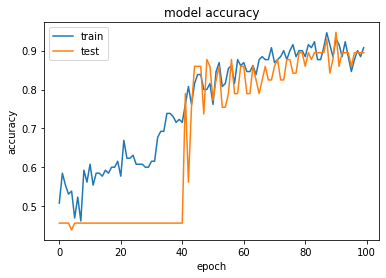
\includegraphics[height=0.35\textwidth]{images/chapter5/batch_256_100_epoch.png} &
        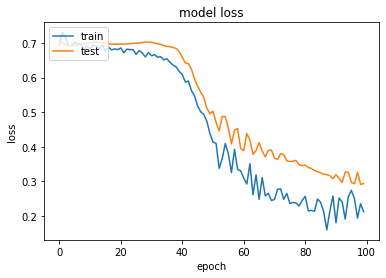
\includegraphics[height=0.35\textwidth]{images/chapter5/batch_256_100_epoch_loss.png}\\
        (a) & (b)\\
    \end{tabular}
    \caption{Resultados de entrenamiento del modelo usando una GPU Tesla K80 con un Batch-size de 256 y 100 Epochs. (a) Rendimiento del modelo en acierto. (b) Rendimiento del modelo en pérdida.}
    \label{fig:100-epochs}
\end{figure}


\subsection{Configuración de 175 Epochs y 256 Batch-size}
 Con un tiempo total de entrenamiento de 25.86 segundos y una precisión del 93\% sobre el conjunto de datos de entrenamiento.
    En las Figuras~\ref{fig:175-epochs} (a) y \ref{fig:175-epochs} (b) se encuentran los resultados de entrenamiento en términos de precisión y pérdida.



    \begin{figure}[H]
    \centering
    \begin{tabular}{cc}
        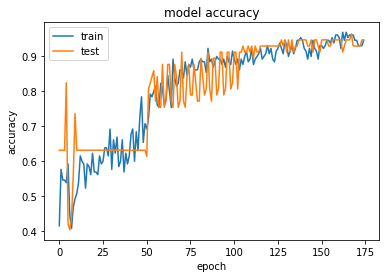
\includegraphics[height=0.35\textwidth]{images/chapter5/batch_256_175_epoch.png} &
        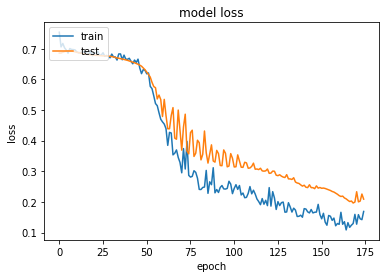
\includegraphics[height=0.35\textwidth]{images/chapter5/batch_256_175_epoch_loss.png}\\
        (a) & (b)\\
    \end{tabular}
    \caption{Resultados de entrenamiento del modelo usando una GPU Tesla K80 con un Batch-size de 256 y 175 Epochs. (a) Rendimiento del modelo en acierto. (b) Rendimiento del modelo en pérdida.}    \label{fig:175-epochs}
\end{figure}

\subsection{Configuración de 200 Epochs y 256 Batch-size}

 Con un tiempo total de entrenamiento de 29.94 segundos y una precisión del 87\% sobre el conjunto de datos de entrenamiento.
    Ver Figuras~\ref{fig:200-epochs} (a) y \ref{fig:200-epochs} (b) para los resultados en precisión y pérdida.




\begin{figure}[H]
    \centering
    \begin{tabular}{cc}
        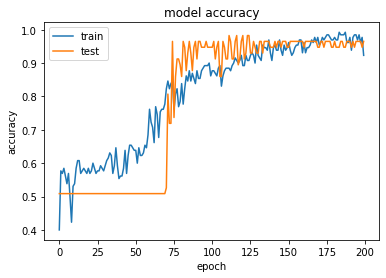
\includegraphics[height=0.35\textwidth]{images/chapter5/batch_256_200_epoch.png} &
        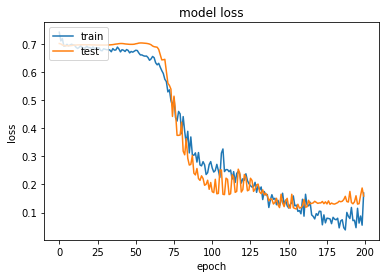
\includegraphics[height=0.35\textwidth]{images/chapter5/batch_256_200_epoch_loss.png}\\
        (a) & (b)\\
    \end{tabular}
    \caption{Resultados de entrenamiento del modelo usando una GPU Tesla K80 con un Batch-size de 256 y 200 Epochs. (a) Rendimiento del modelo en acierto. (b) Rendimiento del modelo en pérdida.}
    \label{fig:200-epochs}
\end{figure}

Podemos observar en la Tabla \ref{tab:Comparativa en el número de Epochs y tiempo de entrenamiento.} que la configuración con 100 Epoch es la que mejor resultado da en cuanto a velocidad, sin embargo, no es la más fiable en cuanto a pérdida del modelo, pudiendo reducir aún más el número de fallos si se aumentan las iteraciones.
Las configuraciones restantes mantienen un nivel alto de predicción. La variante de 200 Epoch al final de su entrenamiento comienza a denotar una tendencia ascendente en el número fallos.
Escogeremos la solución de 175 Epoch al ser más rápida que la de 200 Epoch y más fiable en el número de fallos que la de 100.

\begin{table}[ht]
    \begin{center}
        \begin{tabular}{| c | c | c | c |}
            \hline
            epoch & accuracy & time & loss \\ \hline
            100 & 85\% & 16.79 s & 2.1\% \\
            175 & 93\% & 25.86 s & 1.5\% \\
           200 & 87\% & 29.94 s &  1.9\% \\ \hline
        \end{tabular}
        \caption{Comparativa en el número de Epochs y tiempo de entrenamiento.}
        \label{tab:Comparativa en el número de Epochs y tiempo de entrenamiento.}
    \end{center}
\end{table}

\section{Rendimiento en fase de inferencias}\label{sec:ren-dimiento-en-fase-de-inferencias}
Se han configurado los distintos servidores web para que empleen todos los núcleos del procesador de manera concurrente, de modo que la capacidad de procesamiento de peticiones sea la máxima posible.

Los resultados se presentan haciendo uso de una muestra de 64000 peticiones de inferencia en el entorno de producción de la aplicación, 32000 para la red de TensorFlow y 32000 para la red de OpenVINO.
La unidad de cálculo principal es el procesador, siendo su modelo un Intel Xeon (Cascada Lake) con una frecuencia de 2.8 GHz de base y un turbo hasta 3.4 GHz.

Se han probado distintas configuraciones de este procesador, tanto en su versión de 2 núcleos físicos (4 virtuales), como en la de 4 núcleos físicos (8 virtuales).
La memoria RAM utilizada varía de 4 GB con el procesador de 2 núcleos físicos a 8 GB en la versión de 4 núcleos físicos.

La memoria disponible en todas todas las configuraciones es inferior a la contratada, ya que el total incluye el almacenamiento del sistema operativo y librerías esenciales para su funcionamiento, así como el servicio de Docker.

\subsection{Rendimiento de acierto en la predicción.}
En la Tabla~\ref{tab:Comparativa de acierto de inferencia con OpenVINO y TensorFlow} podemos observar que la tasa de acierto para ambas redes
mantiene un porcentaje de acierto elevado que supera el 97\%. A lo largo de las 32000 inferencias tomadas para cada red se encuentra una diferencia notable en el número de predicciones erróneas. OpenVINO tiene una tasa de error 1.7 veces superior a TensorFlow. Esto es debido a que en OpenVINO se está usando un método de optimización basado en la reducción del tamaño en memoria que ocupan sus variables. En OpenVINO la red de inferencia opera de manera predeterminada con variables en punto flotante de 32 bits, que con el cambio son de 16 bits.
La mejora que nos da esta optimización en la velocidad de inferencia de OpenVINO causa una disminución del potencial de acierto de la red.


\begin{table}[ht]
    \begin{center}
        \begin{tabular}{| c | c | c | c | c |}
            \hline
            inference\_engine & samples & right\_guess & error & percentage\_guess \\ \hline
            OpenVINO & 32000 & 31141 & 859 & 97\% \\
            TensorFlow & 32000 & 31521 & 479 & 98\% \\ \hline
        \end{tabular}
        \caption{Acierto de inferencia en OpenVINO y TensorFlow.}
        \label{tab:Comparativa de acierto de inferencia con OpenVINO y TensorFlow}
    \end{center}
\end{table}

\subsection{Rendimiento en tiempo de inferencia.}
En la Tabla~\ref{tab:Comparativa de tiempo de inferencia con OpenVINO y TensorFlow} se puede observar como la media de inferencia a lo largo de las 64000 muestras tomadas
es de 106 ms para TensorFlow y 3 ms para OpenVINO, lo que supone una velocidad de inferencia 35 veces superior de OpenVINO frente a TensorFlow.

\begin{table}[ht]
    \begin{center}
        \begin{tabular}{| c | c | c | c |}
            \hline
            inference\_engine & samples & avg\_inference\_ms & avg\_ms\_total \\ \hline
            TensorFlow & 32000 & 106 ms & 381 ms \\
            OpenVINO & 32000 & 3 ms & 108 ms \\ \hline
        \end{tabular}
        \caption{Tiempo de inferencia en OpenVINO y TensorFlow.}
        \label{tab:Comparativa de tiempo de inferencia con OpenVINO y TensorFlow}
    \end{center}
\end{table}

El tiempo total de inferencia, que incluye la latencia de la mensajería entre los distintos componentes y el servidor es de 381 ms para TensorFlow y 108 ms para OpenVINO. La solución de OpenVINO no incluye servidores adicionales para su funcionamiento como si hace TensorFlow, por lo que no tiene latencia adicional en este punto.

\subsection{Rendimiento en tiempo de inferencia con distinto hardware.}
Podemos visualizar en la Tabla~\ref{tab:Comparativa de tiempo de inferencia con OpenVINO y TensorFlow con distinto hardware} que el tiempo total de inferencia que incluye la latencia del servidor web, los pipelines de procesamiento del entorno y la propia inferencia, es inferior al segundo en ambos casos.


Las distintas configuraciones hardware también revelan que el consumo de memoria del sistema de inferencia de TensorFlow afecta al rendimiento de la aplicación, mejorando mucho su rendimiento con un hardware más potente.
OpenVINO, por el contrario, mantiene resultados similares con un hardware de bajo coste, con unos resultados de inferencia de 3 ms con el procesador de 2 núcleos y 2 ms con el de 4 núcleos.

\begin{table}[ht]
    \footnotesize
    \begin{center}
        \begin{tabular}{| c | c | c | c | c | c | c |}
            \hline
            inference\_engine & samples & physical\_core & system\_memory & avg\_inference\_ms & avg\_total\_ms \\ \hline
            OpenVINO & 16000 & 2 & 3.46 GB & 3 ms & 87 ms \\
            OpenVINO & 16000 & 4 & 7.00 GB & 2 ms & 128 ms \\
            TensorFlow & 16000 & 2 & 3.46 GB & 146 ms & 521 ms \\
            TensorFlow & 16000 & 4 & 7.00 GB & 67 ms & 241 ms \\ \hline
        \end{tabular}
        \caption{Tiempo de inferencia en OpenVINO y TensorFlow con distinto hardware.}
        \label{tab:Comparativa de tiempo de inferencia con OpenVINO y TensorFlow con distinto hardware}
    \end{center}
\end{table}

Se contempla que el tiempo medio total de inferencia aumenta pese a mejorar el hardware en OpenVINO.
Con el procesador de 4 núcleos tenemos un número total de 8 hilos en el servidor web, el coste de paralelizar las llamadas entre los distintos nodos eleva el coste total de la petición HTTP.

TensorFlow mejora 2 veces la velocidad de inferencia pasando de un procesador de 2 núcleos y 4 GB de RAM a uno de 4 núcleos y 8 GB de RAM teniendo un tiempo de 146 ms con el primero y 67 ms con el segundo, lo que denota que el consumo de su servicio de inferencia requiere de un hardware más potente. Del mismo modo mejora 2 veces su tiempo de inferencia total con la mejora del hardware pasando de 521 ms a 241 ms.

\subsection{Rendimiento en tiempo de inferencia con distinto framework web.}
Es necesario recordar que cada framework web está configurado con un tipo de servidor distinto que pone en marcha su funcionamiento.

Flask se configura junto con el servidor WSGI\footnote{\url{https://linuxgazette.net/115/orr.html}} Gunicorn\footnote{\url{https://gunicorn.org/}}, mientras que FastAPI se configura con el servidor ASGI\footnote{\url{https://channels.readthedocs.io/en/latest/asgi.html}} Uvicorn\footnote{\url{https://www.uvicorn.org/}}. El rendimiento de estos servidores influirá en el tiempo total de la llamada HTTP.

En la Tabla~\ref{tab:Comparativa de tiempo de inferencia con OpenVINO y TensorFlow con distinto framework web} podemos contemplar que OpenVINO se mantiene estable con ambos framework web, con un ligero aumento de la latencia haciendo uso de FastAPI.

TensorFlow se comporta mucho mejor con Flask, mejorando en 2 veces su tiempo de inferencia en la red pasando de 148 ms con FastAPI a 65 ms con Flask y 2 veces en el tiempo total de ejecución teniendo un rendimiento de 517 ms con FastAPI y 246 ms con Flask.

\begin{table}[ht]
    \begin{center}
        \begin{tabular}{| c | c | c | c | c |}
            \hline
            inference\_engine & samples &  web\_engine & avg\_inference\_ms & avg\_total\_ms \\ \hline
            OpenVINO & 16000 & Flask & 2 ms & 103 ms \\
            OpenVINO & 16000 & FastAPI & 3 ms & 112 ms \\
            TensorFlow & 16000 & Flask & 65 ms & 246 ms \\
            TensorFlow & 16000 & FastAPI & 148 ms & 517 ms \\ \hline
        \end{tabular}
        \caption{Comparativa de tiempo de inferencia en OpenVINO y TensorFlow con distinto framework web.}
        \label{tab:Comparativa de tiempo de inferencia con OpenVINO y TensorFlow con distinto framework web}
    \end{center}
\end{table}

Flask es un servidor web con los mínimos componentes para funcionar, pero configurado de la manera correcta puede ser el framework idóneo para realizar una tarea específica.
En este caso, la complejidad del servicio de TensorFlow convive mejor con un framework web sin demasiados componentes adicionales.

Las mejoras que proporciona FastAPI como un sistema de logging detallado de las ejecuciones y algunas características adicionales para el desarrollador\footnote{\url{https://fastapi.tiangolo.com/features/}}, pueden ocasionar cierto aumento de la latencia en los tiempos.
Aun así, cuando la fiabilidad es uno de los requisitos y objetivos principales, estas mejoras pueden valer la pena a la hora de escalar nuestra aplicación.

\subsection{Rendimiento en tiempo de inferencia con distinto framework web y hardware.}
En general, FastAPI requiere de un hardware más potente para sacar su máximo rendimiento, mientras que con un \textit{framework} minimalista como Flask podemos optar por reducir costes en hardware sin penalizar demasiado el rendimiento.

En la Tabla~\ref{tab:Comparativa de tiempo de inferencia con OpenVINO y TensorFlow con distinto hardware y servidor web} podemos ver el rendimiento según hardware, servidor web y sistema de inferencia utilizado.
El sistema de inferencia más rápido en todas las casuísticas es OpenVINO, siendo su configuración con 4 núcleos, 8 GB y Flask la más veloz, con 2 ms de inferencia y 126 ms de procesamiento total de la petición. Esta opción también permite la máxima paralelización de llamadas posibles, al tener consigo los 8 hilos del procesador de 4 núcleos.

\begin{table}[H]
    \begin{center}
        \small
        \begin{tabular}{ | c | c | c | c| c | c | c | c |}
            \hline
            engine & samples & cores & memory & framework & avg\_inference\_ms & avg\_total\_ms \\ \hline
            OpenVINO & 8000 & 2 & 3.46 GB & Flask & 3 ms & 81 ms \\
            OpenVINO & 8000 & 2 & 3.46 GB & FastAPI & 4 ms & 94 ms \\
            OpenVINO & 8000 & 4 & 7.00 GB & Flask & 2 ms & 126 ms \\
            OpenVINO & 8000 & 4 & 7.00 GB & FastAPI & 2 ms & 130 ms \\
            TensorFlow & 8000 & 2 & 3.46 GB & Flask & 64 ms & 221 ms \\
            TensorFlow & 8000 & 2 & 3.46 GB & FastAPI & 229 ms & 821 ms \\
            TensorFlow & 8000 & 4 & 7.00 GB & Flask & 67 ms & 270 ms \\
            TensorFlow & 8000 & 4 & 7.00 GB & FastAPI & 67 ms & 212 ms \\ \hline
        \end{tabular}
    \end{center}
    \caption{Comparativa de tiempo de inferencia en OpenVINO y TensorFlow con distinto hardware y servidor web.}
    \label{tab:Comparativa de tiempo de inferencia con OpenVINO y TensorFlow con distinto hardware y servidor web}
\end{table}




\subsection{Número de peticiones por segundo soportadas por el servidor.}
Se ha tenido en cuenta el rendimiento del framework web, pero no su parte más importante, la paralelización. Es indispensable saber el número de peticiones que podemos soportar por segundo.

Para este experimento (ver Tabla \ref{tab:Peticiones por segundo soportadas por el servidor para OpenVINO y TensorFlow}) se han tomado nuevas muestras para cada sistema de inferencia. La configuración hardware es la más potente posible para ambos casos. Se ha decidido usar el framework de FastAPI ya que su sistema de logging permitirá al desarrollador saber si todas las peticiones enviadas al servidor llegan de manera correcta.
\begin{table}[ht]
    \begin{center}
        \begin{tabular}{| c | c | c | c | c |}
            \hline
            inference\_engine & samples &  seconds & avg\_image\_s & requests\_received\\ \hline
            OpenVINO & 8000 & 119 s & 67 img/s & 8000 \\
            TensorFlow & 8000 & 125 s & 64 img/s & 8000\\ \hline
        \end{tabular}
        \caption{Peticiones por segundo soportadas por el servidor para OpenVINO y TensorFlow.}
        \label{tab:Peticiones por segundo soportadas por el servidor para OpenVINO y TensorFlow}
    \end{center}
\end{table}

El número total de peticiones recibidas por el servidor, en ambos casos, es un 100\% del total de enviadas, por lo que la aplicación soporta con creces este volumen de trabajo.

TensorFlow pese a tener un sistema de inferencia claramente inferior al de OpenVINO es capaz de compensar esta carencia debido a la concurrencia que ofrece el servidor, consiguiendo un rendimiento similar en el tiempo total del procesamiento de todas las imágenes.


Hay que señalar que las dos redes están recibiendo las mismas peticiones por minuto, por lo que puede que alguna no se esté aprovechando del todo y sea capaz de realizar más cálculos por unidad de tiempo.

\subsection{Rendimiento de inferencia en un entorno local.}
Toda la infraestructura que soporta la aplicación acumula latencia en cada conexión que hace entre sus componentes.
Transportar todo este procesamiento a un entorno local, en el que las imágenes ya estén listas para procesar, minimiza el tiempo total de inferencia.
En este punto ponemos a prueba los sistemas de inferencia sin herramientas que puedan generar ruido.
Para esta prueba hemos conservado el hardware más potente que usábamos en los servidores web: un procesador con 4 núcleos físicos y 8 GB de memoria RAM.

Como podemos observar en la Figura \ref{fig:TensorFlow VS OpenVINO}, se reafirman los resultados obtenidos en las pruebas de rendimiento de inferencia en el pipeline del servidor. OpenVINO es mucho más rápido calculando los resultados de las predicciones. Es en este entorno donde podemos ver el verdadero potencial de usar un lenguaje de bajo nivel. Esto nos permite gestionar operaciones en memoria, manipular el borrado de variables que ya no se necesitan, elegir el número de BYTES que ocupan nuestras estructuras de datos.
El poder de decisión que nos brindan estas ventajas se convierten en rendimiento cuando ponemos a prueba nuestra aplicación.
En este entorno conseguimos una tasa de 541 img/s para OpenVINO y 39 img/s para TensorFlow. Sin la gestión de concurrencia que proporciona el servidor web la diferencia es notable. TensorFlow no ofrece una rápida inferencia unitaria, por lo que su capacidad de procesamiento no es la mejor en este entorno.

\begin{figure}[H]
    \centering
        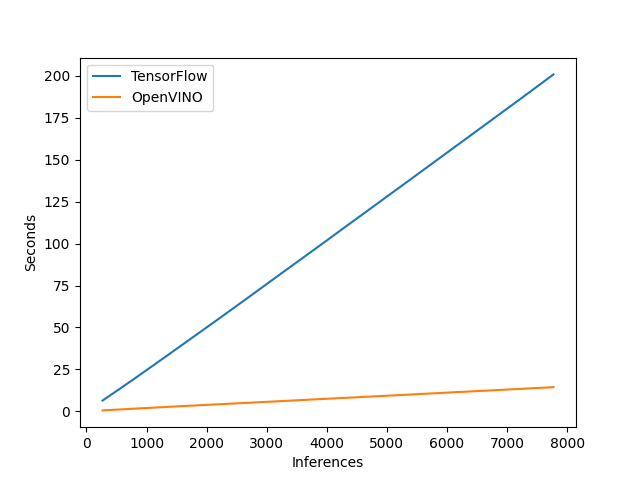
\includegraphics[height=0.5\textwidth]{images/chapter5/local_inferences.png} &
    \caption{Comparativa de inferencias entre TensorFlow y OpenVINO en un entorno local.}   \label{fig:TensorFlow VS OpenVINO}
\end{figure}

Todos los resultados y registros se encuentran en el repositorio oficial del trabajo en GitHub\footnote{\url{https://github.com/A-Ortiz-L/multispectral-imaging-cnn-final-degree-work/tree/master/result/snapshot}}.

\section{Costes del proyecto}\label{sec:costes-del-proyecto}
A continuación se presentan los costes del proyecto de toda la plataforma de producción.
La suma total durante todo el desarrollo del proyecto del entorno productivo es de 10.20 dólares.
Estos costes han sido recogidos haciendo uso de la calculadora de precios de Google\footnote{\url{https://cloud.Google.com/products/calculator?hl=es}}.

\begin{itemize}
    \item Máquina virtual 4 núcleos y 4 GB de memoria RAM. Un total de 6.80 dólares por un uso de 24 horas, que fue el tiempo utilizado para realizar pruebas de concepto y cargas en este trabajo.
    \item Máquina virtual 2 núcleos y 4 GB de memoria RAM. Un total de 3.40 dólares por un uso de 24 horas, que fue el tiempo real consumido para este servicio.
    \item BigQuery, con un coste de 0.00 dólares para un almacenamiento de 1 GB de tablas en la base de datos, 1 GB de procesamiento en tiempo real y 1 GB de trabajos SQL al realizar los análisis de resultados.
    \item Pub/Sub con un coste total de 0.00 dólares, ya que su uso entraba dentro del rango gratuito del servicio.
    \item Cloud Functions, con un coste total de 0.00 dólares, haciendo uso de la modalidad gratuita, que permite hasta 2 millones de llamadas al mes.
\end{itemize}

Según la calculadora de salarios de Stack Overflow\footnote{\scriptsize\url{https://stackoverflow.blog/2019/10/16/coding-salaries-in-2019-updating-the-stack-overflow-salary-calculator/}}, el salario bruto de un ingeniero \textit{Data Scientist} \textit{junior} en Madrid, que maneja herramientas como Docker, Google Cloud Platform, Python, TensorFlow y SQL, puede rondar los 28000 y 42000 euros brutos al año.

El total de semanas consumidas en la consecución de este proyecto es de diez.
Suponiendo un salario bruto de 28000 euros anuales, un desarrollador tendría que estar contratado durante diez semanas a jornada completa para la elaboración del proyecto, lo que resultaría en un total de 5832 euros.
